\chapter{Scheme and design of the Mobile library and the Desktop tool}
 
The main goal and the main subject of this thesis is to create an end-to-end computer vision pipeline that allows developers to build applications for mobile phones that utilize computer vision to detect game objects through the camera. The final applications should look something like this:

\begin{figure}[hbt]
	\centering
	\includegraphics[width=0.7\textwidth]{obrazky-figures/final_result_scheme.pdf}
	\caption{Result application detecting cards for a card game Bang!}
	\label{ResultApplicationScreenshot}
\end{figure}

The figure above shows a mobile application detecting game objects, in this case, cards from the game Bang!. Design choices, such as colors, rounded corners, navigation menus, etc., should be left up to the developers. However, the underlying layer, which works with the camera and neural networks that detect these objects, should provide an interface for developers to build on top of. 

Furthermore, during the initial development of the application, I, as the author, encountered obstacles that slowed down the process of creating a demonstrative application. These problems were mostly related to gathering and annotating image data, as well as training neural networks that detect these objects. This is the crucial step for all applications, as the datasets containing annotated image data, let alone finished neural networks, might not always be available to the developers, and they may be forced to create them from scratch.

Because of that, an application that would help provide at-least basic functionality was proposed as part of the solution. This application will provide functionality to build these models from scratch, even if they are not the most efficient. These models can later be used by the mobile library for object detection tasks. Therefore, it is crucial to use a format for these models so that inexperienced developers will be able to use both both mobile library and the application with ease, while leaving just enough space for advanced developers to modify these models and the way they are handled to their liking, should they desire. 

\begin{figure}[hbt]
	\centering
	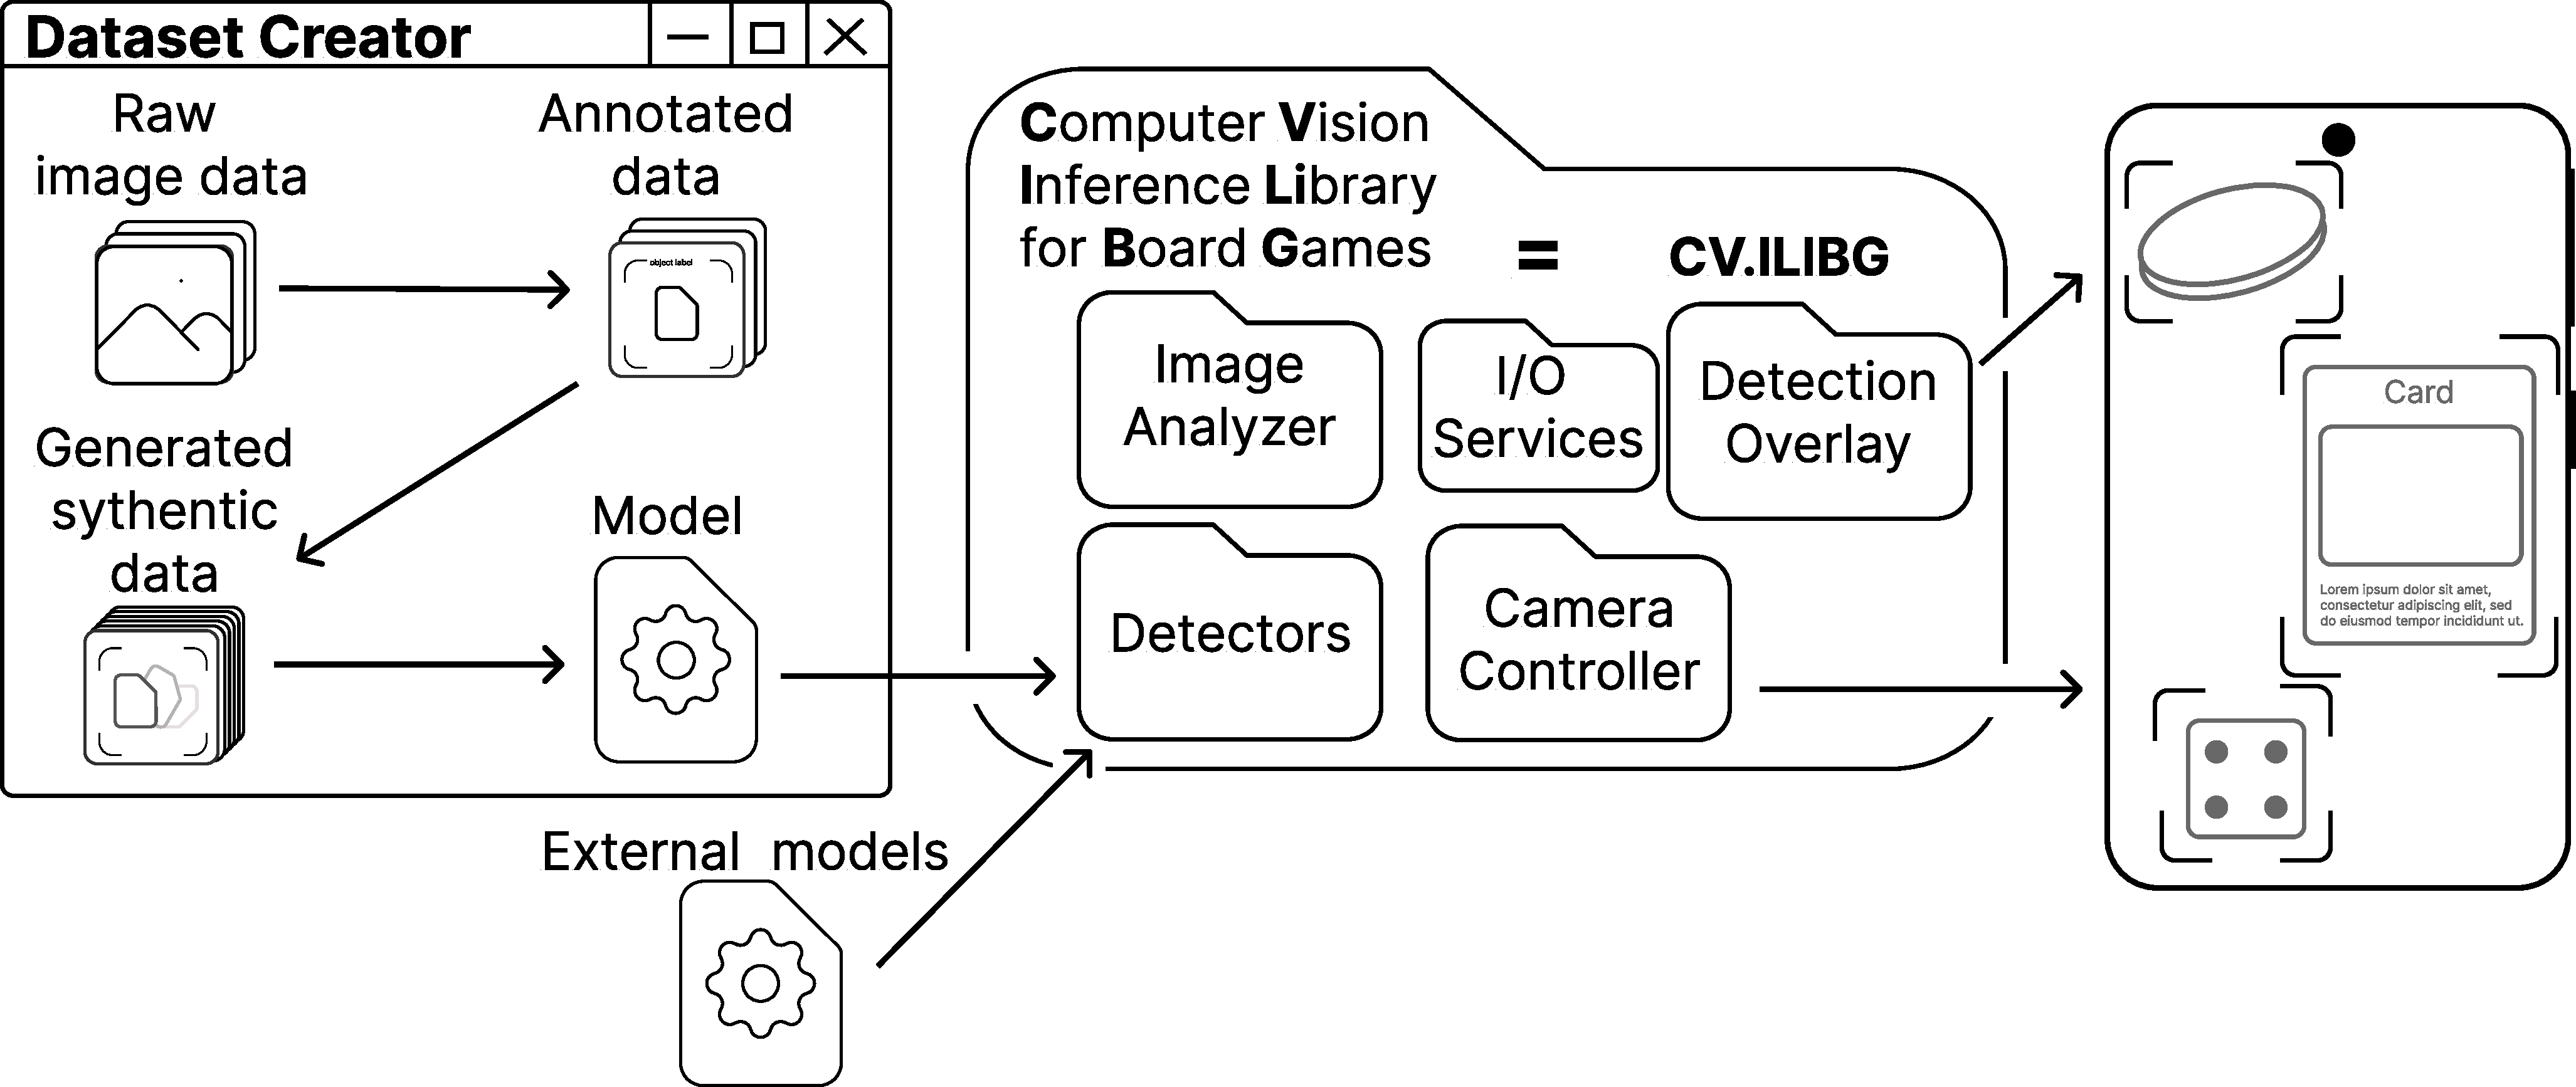
\includegraphics[width=0.98\textwidth]{obrazky-figures/project_scheme.pdf}
	\caption{Scheme of project structure.}
	\label{ProjectScheme}
\end{figure}

\textbf{Dataset Creator} on the left side provides a way for developers to transform raw image data into functional models for object detection. While the application can work with the models provided by the \textbf{Dataset Creator}, it must also provide some interface for developers to adapt other \textit{"External"} models to work with the library. The mobile library in the middle handles camera, input/output services, object detection, displaying detected objects onto the devices screen, and a bunch of other smaller repetitive tasks. 
